\chapter{Grundlagen}
\label{chap:grundlagen}
    In diesem Kapitel werden die für diese Thesis relevanten Grundlagen geschaffen, um ein Grundverständnis und 
    fundiertes Wissen über verwendete Technologien zu erlangen und die nachfolgende Recherche, Konzeption und 
    Umsetzung besser verstehen zu können. 

\section{Internet der Dinge}
\label{sec:iot}
    Das \ac{IdD}, im Englischen \ac{IoT}, zählt als eines der Schlagworte in der \ac{IT}. In der Domäne des \acs{IoT} bekommen 
    Gegenstände und Objekte eine eindeutige Identität, die eine Kommunikation miteinander als auch das Entgegennehmen von 
    Befehlen erlaubt. Mit dem \acl{IdD} lassen sich Anwendungen sowie Prozesse automatisieren und Aufgaben erledigen ohne das 
    von außen Eingegriffen werden muss \cite{bigdatainsider2016}. Die Prozessautomatisierung findet sich auch im Kontext des 
    \acl{SH} wieder, welches in nachfolgendem Kapitel genauer aufgegriffen wird. 
    \\
    \linebreak
    In der einschlägigen Literatur gibt es für das \acl{IoT} keine allgemeingültige Definition, die alle Anwendungsbereiche abdeckt. 
    Die Definitionen und Auslegungen der Interpretation unterscheiden sich je nach Anwendungsgebiet. Demnach gibt es viele verschiedene 
    Forschungsgruppen, darunter Forscher, Akademiker, Innovatoren, Entwickler und Geschäftsleute, die den Begriff oder die zugrundeliegende 
    Problemstellung definiert haben. Die Ursprünge jedoch sind dem Experten für digitale Innovationen, 
    Kevin Ashton\footnote{Britischer Technologie-Pionier, Mitgründer des Auto-ID Centers am Massachusetts Institute of Technology (MIT). \url{https://de.wikipedia.org/wiki/Kevin_Ashton} (Abgerufen am 22.03.2022)}, 
    zuzuschreiben. 
    \\ 
    Die in der Literatur auffindbaren Definitionen verfolgen zwei Sichtweisen. Zum einen die aktive Sicht, d. h. 
    die Daten sind von Menschen erstellt, zum anderen die passive, bei der die Daten von Dingen, darunter die Sensoren und Aktoren, 
    erstellt werden \cite{Madakam2015}. Eine aus dem Zusammenhang hervorgehende, aus dem wissenschaftlichen Artikel entnommene 
    Definition ist folgende:
    % „Ein offenes und umfassendes Netzwerk intelligenter Objekte, die in der Lage sind, sich automatisch zu organisieren, 
    % Informationen, Daten und Ressourcen auszutauschen und auf Situationen und Veränderungen in der Umgebung zu reagieren 
    % und zu handeln.“
    \pagebreak
    \begin{quote}
        “An open and comprehensive network of intelligent objects that have the capacity to auto-organize, share information, data 
        and resources, reacting and acting in face of situations and changes in the environment” \cite{Madakam2015}
    \end{quote}
    Daraus kann die Ableitung erfolgen, dass der Begriff des \acl{IdD} für die Vernetzung von Gegenständen im privaten Gebrauch, sowie 
    von industriellen Geräten und Maschinen über das Internet, steht. Damit Geräte individuell angesprochen werden können, werden diese 
    mit einer eindeutigen Identität, genauer einer \ac{IP}-Adresse, im Netzwerk belegt und mit elektronischer Intelligenz ausgestattet \cite{bigdatainsider2016}.
    Darüber können die Netzwerkteilnehmer über das Internet kommunizieren und Prozesse automatisiert erledigen. Die sogenannten 
    \textit{intelligenten Geräte} werden auch oft mit dem englischen Begriff, \textit{Smart Devices}, betitelt. 
    \\
    \linebreak
    Neben der Kommunikation der Geräte über das Netzwerk untereinander kann ebenso entweder über das Gerät selbst oder eine zentrale 
    Schnittstelle über das Internet interagiert werden. Dadurch sind Objekte und Gegenstände durch einen Benutzer von beliebigen Orten 
    auch außerhalb des Netzwerks erreichbar und können so bedient werden. Diese Art und Weise wird auch in dem zentralen Thema des 
    \acl{SH} verwendet. Die Funktion als auch die Umsetzung wird im Kapitel (\ref{sec:smartHome}) näher beleuchtet.
    \\
    \linebreak
    Das \acl{IdD} ist ein nahezu existenzielles Konzept der \acs{IT}-Welt. Mit dem \acs{IoT} wird die Vision verfolgt, eine globale 
    Infrastruktur zu erstellen, mit der physische Objekte miteinander vernetzt werden und jeder Zeit zur Verfügung stehen. Das \acl{IoT} 
    kann auch als globales Netzwerk angesehen werden, indem die Kommunikation zwischen Mensch zu Mensch, Gerät zu Mensch und Gerät zu 
    Gerät ermöglicht wird. Viele Forschungsartikel sprechen von der Verschmelzung der digitalen und 
    der physischen Welt.\footnote{Das Internet der Dinge – der digitale Zwilling der Welt. Kompetenzzentrum Öffentliche IT in Kooperation mit dem Fraunhofer Institut. \url{https://www.oeffentliche-it.de/trendsonar-iot} Abgerufen am 23.03.2022.} 
    Die Vereinigung beider Welten ist die Verknüpfung physischer Objekte, die eindeutig identifizierbar sind, mit einer virtuellen 
    Repräsentation in einer vergleichbaren Internet-Struktur. 
    \subsection*{Gesamtbild des \acl{IoT}}
        Der folgenden Abbildung (\ref{pic:mindmap_IoT}) ist zu entnehmen, welche Technologien rund um das \acl{IdD} liegen und in Verbindung damit stehen. 
        \begin{figure}[hbt!]
            \centering
            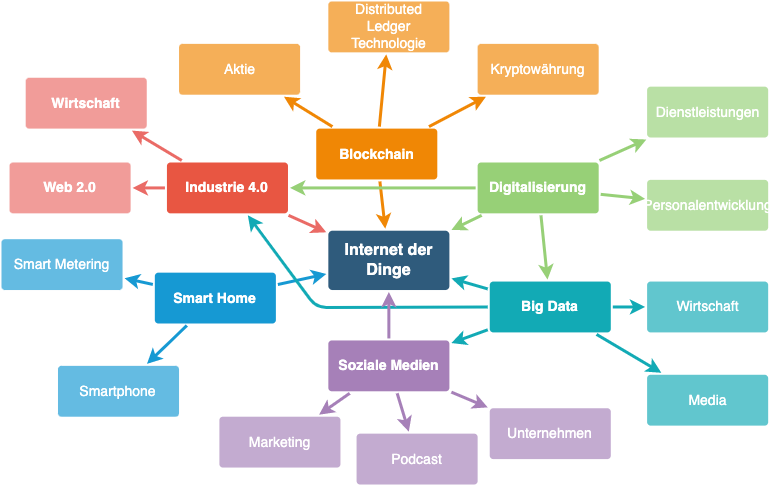
\includegraphics[width=15cm,height=15cm,keepaspectratio]{images/IoT-Mind_Map.png}
            \caption{Technologische Einordnung von IoT \cite{iotmindmap2018}}
            \label{pic:mindmap_IoT}
        \end{figure}
        \\
        \pagebreak
        \linebreak
        Beispielsweise ist das \acs{IoT} eine wesentliche Grundlage für das Themengebiet \textit{Big Data}. Die durch Sensoren 
        und Aktoren erzeugten Daten 
        können Grundlage für die Verwendung im Bereich \textit{Big Data} sein. Dabei werden die Datenmengen gespeichert und mithilfe von Mustern 
        und Herangehensweisen des Big Data\footnote{Definition und Funktionsweise von Big Data. \url{https://www.oracle.com/big-data/what-is-big-data/} Abgerufen am 25.03.2022} 
        analysiert. 
        Big Data ist kein Bestandteil dieser Arbeit und wird demnach nicht weiter ausgeführt. Das Beispiel dient lediglich zu Veranschaulichung 
        und Interpretation der oben aufgeführten Abbildung (\ref{pic:mindmap_IoT}).
        \\
        \linebreak
        Eine allgemeine exemplarische Skizzierung eines Systems, welches nach dem \acs{IoT}-Konzept aufgebaut ist, kann der folgenden 
        Abbildung (\ref{pic:skizze_iot}) entnommen werden:
        \begin{figure}[hbt!]
            \centering
            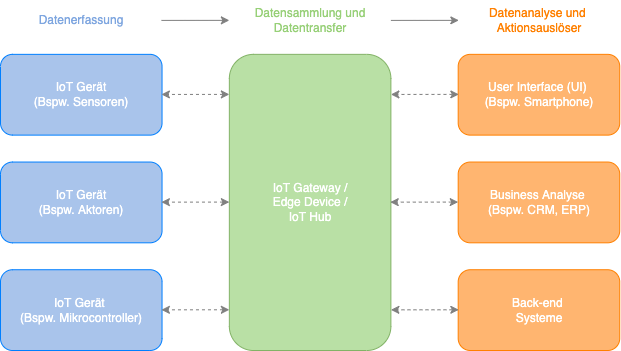
\includegraphics[width=15cm,height=15cm,keepaspectratio]{images/IoT_Grundstruktur.png}
            \caption{Exemplarische Darstellung eines \acs{IoT}-Systems \cite{iotskizze2022}}
            \label{pic:skizze_iot}
        \end{figure}
        \\
        \pagebreak
        \linebreak
        Hierbei werden die jeweiligen Komponenten verdeutlicht, die in einem System zu finden sind. Mit den \textit{IoT-Geräten}, darunter 
        beispielsweise Sensoren und Aktoren, findet die Datenerzeugung statt. Mit dem dahinterstehenden \textit{Gateway} werden die aus den Geräten 
        erzeugten Daten gesammelt und an zentraler Stelle an die Cloud gesendet. Nach der Datensammlung können diese an verschiedene 
        Komponenten zur weiteren Verarbeitung gesendet werden. Sie kann durch Visualisierung über das Smartphone stattfinden oder zur Durchführung von 
        Prozessanalysen. Ebenso können die Daten an weitere Backend-Systeme zur Weiterverarbeitung übermittelt werden. 
        
    \subsubsection*{Anwendungsbereiche des \acs{IoT}}
        Grundlegend können im Bereich des \acl{IoT} zwischen zwei Anwendungsbereichen unterschieden werden, zum Einen im privaten Bereich und zum 
        Anderen im industriellen Bereich. Der private Bereich deckt hauptsächlich die Thematik rund um den Gebrauch von Alltagsgegenständen ab und 
        deren Vernetzung untereinander, um eine komfortablere und intelligentere Nutzung der Geräte zu ermöglichen. Darin inbegriffen sind 
        Gebäudeautomatisierungen und die Ereignissteuerung über das Internet. Diese Funktionen sind Hauptbestandteil des \acl{SH}-Konzeptes, welches 
        in Abschnitt (\ref{sec:aufbau}) genauer aufgegriffen wird. 
        \\
        \linebreak
        Der industrielle Bereich beschäftigt sich damit, Maschinen und Anlagen so miteinander zu vernetzen, dass sich ganze industrielle Prozesse 
        automatisiert lassen und so die Effizienz der Prozess- und Produktionsabläufe steigern. Die Nutzung des \acs{IoT} im industriellen Bezug 
        ist ein elementarer Bestandteil der heutigen \textit{Industrie 4.0}\footnote{Definition und Beschreibung der Industrie 4.0 \url{https://www.plattform-i40.de/IP/Navigation/EN/Industrie40/WhatIsIndustrie40/what-is-industrie40.html} Abgerufen am 25.03.2022}.
        Eine genauere Benennung dieser Sparte ist oft auch unter dem \textit{\ac{IIoT}} bekannt. An dieser Stelle wird zwischen den beiden Anwendungsbereichen 
        stark differenziert, da im Rahmen dieser Arbeit lediglich der Fokus auf dem privaten Bereich des \acs{IoT} liegt. 
        \\
        \linebreak
        Mit dem \acl{IdD}-Ansatz gibt es zwei Paradigmen, die in Kombination als auch alleinstehend Anwendung finden. Diese werden in folgendem Abschnitt kurz erläutert.

        \subsubsection*{Edge und Cloud Computing}
            Bei den beiden Paradigmen handelt es sich zum Einen um Edge Computing und zum Anderen um Cloud Computing. Ziel beider Ansätze ist das 
            Verwalten von Daten, bzw. das Arbeiten mit erzeugten Daten
            \\
            Das Edge Computing verfolgt einen \textit{dezentralen Ansatz}, bei dem die Berechnung und Haltung der Daten näher bei der Datenerzeugung gehalten wird. 
            Dies bedeutet, dass jedes Gerät über eine eigene Intelligenz verfügt, bei der Daten direkt nach der Erzeugung verarbeitet und gespeichert werden können. 
            Zu späterem Zeitpunkt kann in From einer Datenbündelung oder einer Vorauswahl die Informationen an ein Rechenzentrum weitergegeben werden. 
            \begin{quote}
                “Edge computing is different from traditional cloud comput- ing. It is a new computing paradigm that performs computing at the edge 
                of the network. Its core idea is to make computing closer to the source of the data [...]” \cite{Cao2020}
            \end{quote}
            Bei Cloud Computing handelt es sich grundlegend um die Bereitstellung von Computerdiensten, Rechenleistung, Ressourcen und Kapazitäten über 
            das Internet, die nicht in einem eigenen Rechenzentrum 
            verwaltet und betrieben werden müssen. Die Verwaltung wird der Anbieter des Cloud Computing überlassen. Hauptsächlich steht dabei die 
            flexible Ressourcennutzung, Skalierung und Verteilung von Rechenleistung im Vordergrund. In Zusammenhang mit den Verfügbaren Ressourcen 
            werden auch verschiedene Modelle, Cloud Typen und diverse Dienste angeboten\footnote{Einblick in die Cloud-Umgebung von dem Anbieter Microsoft. \url{https://azure.microsoft.com/en-us/overview/what-is-cloud-computing/} Abgerufen am 28.03.2022}. 
            Diese werden ihm Rahmen der Arbeit nicht weiter ausgeführt.
            \begin{quote}
                “Cloud computing is a model for enabling ubiquitous, convenient, on-demand network access to a shared pool of configurable 
                computing resources (e.g., networks, servers, storage, applications, and services) that can be rapidly provisioned and 
                released with minimal management effort or service provider interaction.” \cite{Mell2011}
            \end{quote}
            Mit dem Cloud Computing wird im Vergleich zum Edge Computing ein zentraler Ansatz verfolgt, bei dem die erzeugten Daten von den Aktoren und 
            Sensoren direkt an eine zentrale Stelle gelangen, an der auch die Verarbeitung und Analyse der Daten stattfindet. 
            \\
            Eine Kombination beider Ansätze verbindet die stärken und ist als \textit{Hybrid Cloud} bekannt. Diese Konstellation ist in den meisten 
            Architekturen wiederzufinden. 
    
    \subsection{Paradigmen und Kommunikationsmodelle}
        Damit eine umfassende Grundlage im Bereich \acs{IoT} geschaffen wird, behandelt folgender Abschnitt Paradigmen und Kommunikationsmodelle, die 
        in dieser Umgebung verwendet werden. Für die Darstellung dieser Modelle wird eine Literaturquelle genutzt, mit der ein paar der gängigsten und 
        prägnantesten Architekturen und Modelle in diesem Segment abgedeckt sind. Die Repräsentation der Interaktionsparadigmen sind den Schaubildern 
        (\ref{pic:interactionparadigm}) zu entnehmen. 
        \begin{figure}[hbt!]
            \centering
            \begin{subfigure}[b]{0.4\textwidth}
                \centering
                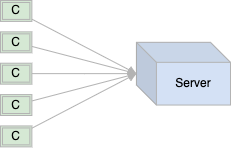
\includegraphics[width=6cm,height=6cm,keepaspectratio]{images/C-S.png}
                \caption{Client-Server Paradigma}
                \label{pic:cs}
            \end{subfigure}
            \begin{subfigure}[b]{0.4\textwidth}
                \centering
                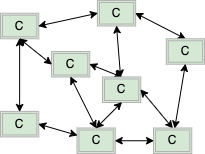
\includegraphics[width=6cm,height=6cm,keepaspectratio]{images/PtoP.png}
                \caption{Peer to Peer Paradigma}
                \label{pic:pp}
            \end{subfigure}
            \begin{subfigure}[b]{0.4\textwidth}
                \centering
                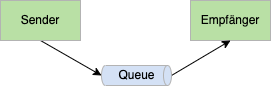
\includegraphics[width=7.5cm,height=7.5cm,keepaspectratio]{images/messagepassing.png}
                \caption{Message Passing Paradigma}
                \label{pic:messagepassing}
            \end{subfigure}
            \caption{Client-Server, Peer-to-Peer und Message Passing Interaktionsparadigma \cite{IEEE2015}}
            \label{pic:interactionparadigm}
        \end{figure}
        \\ 
        \begin{table}[hbt!]
            \begin{center}
                \begin{tabular}{| p{3cm} | p{12.75cm} | }
                    \hline
                        \textbf{Name} & \textbf{Beschreibung} \\
                    \hline
                        Client-Server (\ref{pic:cs}) & Basierend auf einer sehr einfachen Interaktion zwischen Clients und dem Server. Ein Client sendet eine Anfrage an den Server und erwartet dementsprechend eine Antwort. \\ 
                    \hline
                        \ac{PP} (\ref{pic:pp}) & Gegensatz zu Client-Server Konzept. Hierbei können Geräte sowohl als Client Dienste abfragen, als auch als Server Dienste anbieten. \\ 
                    \hline
                        Message Passing (\ref{pic:messagepassing}) & Basierend auf einer einfachen Organisation in der ein Absender eine Nachricht mittels einer Warteschlange (Queue) an einen Empfänger weiterleitet. \\ 
                    \hline
                \end{tabular}
            \end{center}
            \caption{Interaktionsparadigmen nach \cite{IEEE2015}}
            \label{table:kommunikationdmodelle}
        \end{table}
        \\
        \pagebreak
        \linebreak
        Eine Analyse und detailliertere Darstellung der jeweiligen Ansätze kann der Ausarbeitung, aus der die Paradigmen verwendet wurden, entnommen werden.
        \\
        \linebreak
        In Zusammenhang mit Architekturen, die in dem Bereich \acs{IoT} Anwendung finden, und den Interaktionsparadigmen wird häufig zur Unterstützung 
        verschiedener Interaktionsmodelle auf Protokolle gesetzt, die Daten und Primitiven transportieren. Diese Kommunikationsmodelle sind in zwei 
        Bereiche, die ihre Anwendung in \ac{MtoM} finden, kategorisiert:
        \\
        \begin{itemize}
            \item \ac{SOAP}\footnote{Detailliertere Definition des Begriffs SOAP. \url{https://www.redhat.com/en/topics/integration/whats-the-difference-between-soap-rest} Abgerufen am 29.03.2022}: 
            Dabei handelt es sich um ein Standardprotokoll, dass dafür entwickelt wurde, 
            um verschiedene Programmiersprachen auf verschiedenen Plattformen untereinander 
            kommunizieren zu lassen.
            \item \ac{REST}\footnote{Detailliertere Definition des Begriffs REST. \url{https://www.redhat.com/en/topics/integration/whats-the-difference-between-soap-rest} Abgerufen am 29.03.2022}: 
            Dabei handelt es sich um eine Reihe von Architekturprinzipien, die auf 
            die Anforderungen leichtgewichtiger Webdienste und mobiler Anwendungen abgestimmt sind. 
            Anfragen, die über diese Form gesendet werden, können in mehreren Formaten beantwortet 
            werden, darunter beispielsweise \ac{HTML}, \ac{XML} und \ac{JSON}.
        \end{itemize}
        Beide verfolgen das Ziel der Datenübermittlung zwischen Web-Anwendungen über eine Schnittstelle, das sogenannte \ac{API}.
        \acs{REST} Architekturen werden bei einem \acs{IoT}-Szenario aufgrund ihrer Einfachheit und ihrer Bequemlichkeit 
        in einer beschränkten Umgebung bevorzugt. \cite{IEEE2015} 

    \subsection{Historische Entwicklung}
        Die ersten Konzepte zu dem heute bekannten \acs{IoT} liegen schon einige jahrzehnte zurück. 
        Die historische Definition des \acl{IoT} wurde im Jahr 1999 von Kevin Ashton geprägt. Von der 
        Definition bis hin zum erstmaligen Einsatz, bzw. zur Umsetzung eines Konzepts vergingen noch 
        ein paar Jahre. Ein kurzer Einblick in die chronologische Entstehung des \acs{IoT} ist der 
        folgende Tabelle zu entnehmen: 
        \begin{table}[hbt!]
            \begin{center}
                \begin{tabular}{| p{3cm} | p{12.75cm} | }
                    \hline
                        \textbf{Jahr} & \textbf{Industrielle Beteiligung und Zuordnung} \\
                    \hline
                        1970 & Der erste Vorschlag zu miteinander verbundenen Geräten und Maschinen \\ 
                    \hline
                        1990 & John Romkey und Simon Hackett entwickelten den ersten Toaster, der über das Internet an- und ausgeschaltet werden konnte.\footnote{Geschichte to Romkey. \url{https://www.livinginternet.com/i/ia_myths_toast.htm} Abgerufen am 30.03.2022.} \\ 
                    \hline
                        1995 & Das Unternehmen Siemens leitete das erste Mobilfunkmodul ein, welches für die Kommunikation zwischen Maschinen zuständig ist (\acs{MtoM}-Technologie).\\ 
                    \hline
                        1999 & Die Definition des Begriffs \acs{IoT} von Kevin Ashton wurde veröffentlicht und von der Gesamtheit akzeptiert, als er bei \ac{PG} an den sogenannten \ac{RFID} Chips arbeitete. \acs{RFID}-Chips verwenden elektromagnetische Felder, die an Objekte angebracht sind, um diese identifizieren und verfolgen zu können. Ein solches System besteht aus einem Funktransponder, einem Funkempfänger und -sender. \\ 
                    \hline
                        2004 - 2005 & Der Begriff wurde in angesehenen Publikationen verwenden, darunter dessen von Boston Globe und The Guardian. \ac{ITU} veröffentlichte deren ersten Bericht über das Thema. \\ 
                    \hline
                        2008 - 2011 & Die Definitionen und Publikationen fanden erste Anwendungen in praktischen Umsetzungen. Gartner Inc. nahm den Begriff in ihre Recherche-Arbeiten mit auf. \\ 
                    \hline
                \end{tabular}
            \end{center}
            \caption{Historische Entwicklung vom \acl{IdD} \cite{Durga2020}}
            \label{table:iothistory}
        \end{table}
        \\
        \pagebreak
        \linebreak
        Mittlerweile ist das \acl{IdD} ein fester Bestandteil der Industrie und auch im privaten Umfeld. Viele 
        Szenarien und Konzepte werden erarbeitet und umgesetzt. Die Kommunikation von Maschinen untereinander 
        ist in der heutigen Zeit nicht mehr wegzudenken. Forschergruppen sind stark daran interessiert, mehrere 
        Gebiete und Anwendungsbereiche innerhalb des \acs{IoT} zu erforschen. Stark vertreten ist dabei das \ac{FraunhoferIIS}

    \subsection{Ziele von \acs{IoT}}
    \label{subsec:ziele-iot}
        Die Definition von dem \acl{IdD} gibt schon die Richtung an, in die sich die Zielsetzung von 
        \acs{IoT} bewegt. Davon ist das Ziel abzuleiten, dass die Lücke zwischen der realen und der 
        virtuellen Informationswelt so gering wie möglich gehalten, bzw. zunehmend minimiert wird. 
        Dieser Informationsbedarf oder auch die Informationslücke besteht, da in der realen Welt Objekte, 
        Dinge und Gegenstände einen bestimmten Zustand haben, z.B. „die Temperatur liegt bei 35 Grad Celsius“ 
        oder „das Licht ist an und hat 75 \% Helligkeit“, die in der virtuellen Welt nicht verfügbar sind. 
        Das verfolgte Ziel demnach, welches auch zum Großteil im Bereich \acl{SH} abgedeckt wird, ist, dass 
        viele reale Gegenstände ihre Zustandsinformationen für die Weiterverarbeitung in der virtuellen 
        Welt, beziehungsweise im Netzwerk zur Verfügung stellen. Diese Informationen können beispielsweise 
        Aussagen zu der aktuellen Nutzung, der Bedingungen an einer bestimmten Stelle oder Uhrzeit und 
        über Alterung geben. Diese Zustandsinformationen können dazu beitragen, dass die Nutzung des 
        Gegenstandes vom Anwender ausgewertet und so optimiert werden kann, z.B. durch die Erkennung 
        eines Defekts oder einer Automatisierung, damit die Ressource effizient genutzt wird. 

        %In einem weiteren Schritt können digitale Services als Teil des IoT die Parametrierung von 
        %Geräten so erleichtern und verbessern, dass sie auch dort geschieht, wo sie heute aus 
        %Kostengründen nicht stattfindet. Wichtige Schritte zu diesem Ziel sind:

        %die Standardisierung der Komponenten und Dienste im Internet der Dinge;
        %die Einführung einer einfach zugänglichen, sicheren und allgemeinen Netzwerkanbindung, geeignet für alle Geräte mit eingebautem Mikrocontroller;
        %die Reduktion der Kosten für in das IoT integrierte Teilnehmer (Gerätekosten, Inbetriebnahmekosten, Anschlusskosten etc.);
        %die Entwicklung von kostenarmen, automatisierten (bis hin zu autonomen) digitalen Services im Netzwerk, die den zusätzlichen Nutzen der Vernetzung realisieren.